%\subsection{Combining BF and PLR in LSM-tree}
\subsection{Tree Organization and Its Impacts}
%Combining BF and PLR in LSM-tree}
\label{sec:design:tree}
\begin{figure}[t]
\centering
     \begin{subfigure}[b]{0.21\textwidth}
         \centering
         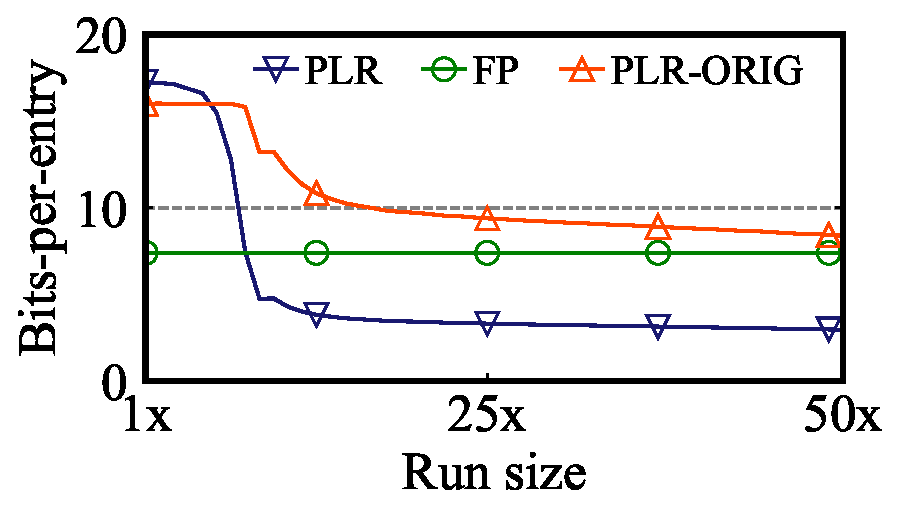
\includegraphics[width=\textwidth]{figs/OSDI/exp_data/bit-per-entry/OURS-BF-PLR.eps}
         \vspace{-10pt}
         \caption{\# of bits per entry}
     \end{subfigure}
     \hfill
     \begin{subfigure}[b]{0.21\textwidth}
         \centering
         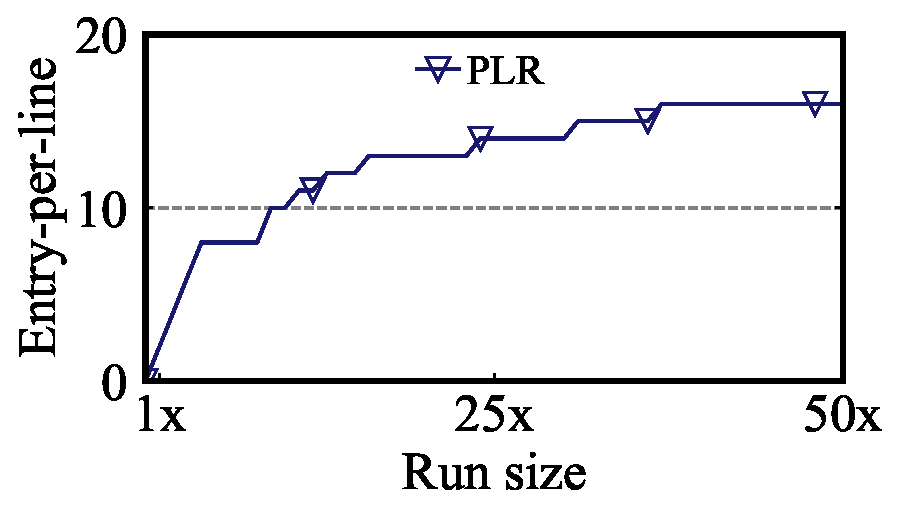
\includegraphics[width=\textwidth]{figs/OSDI/exp_data/line-per-entry/PLR-Range.eps}
         \vspace{-10pt}
         \caption{\# of entries per line}
     \end{subfigure}
       \vspace{-10pt}
     \caption{Memory usage of FP and FPR depending a run size}
%     \caption{\fixme{\# of bits per entry and \# of entries per line in PLR}}

     \label{fig:bf-plr-bit}
\end{figure}




\begin{comment}
\begin{figure*}[t]
     \centering
     \begin{subfigure}[b]{0.175\textwidth}
         \centering
         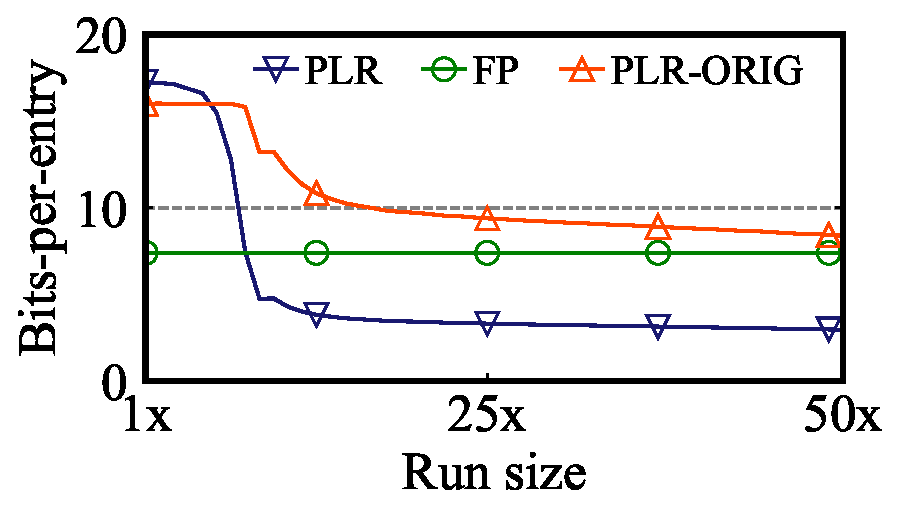
\includegraphics[width=\textwidth]{figs/OSDI/exp_data/bit-per-entry/OURS-BF-PLR.eps}
         \caption{\# of bits per entry}
     \end{subfigure}
     \hfill
     \begin{subfigure}[b]{0.175\textwidth}
         \centering
         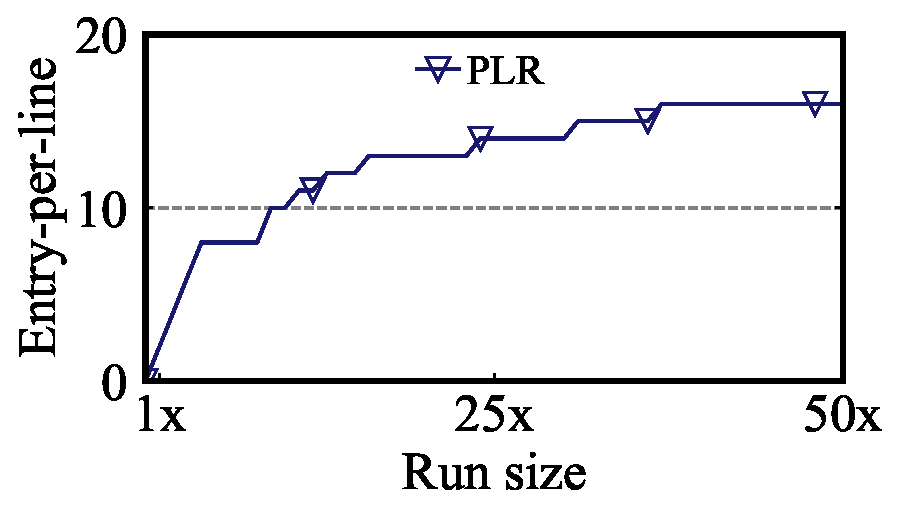
\includegraphics[width=\textwidth]{figs/OSDI/exp_data/line-per-entry/PLR-Range.eps}
         \caption{\# of entry per line}
     \end{subfigure}
     \hfill
     \begin{subfigure}[b]{0.28\textwidth}
         \centering
         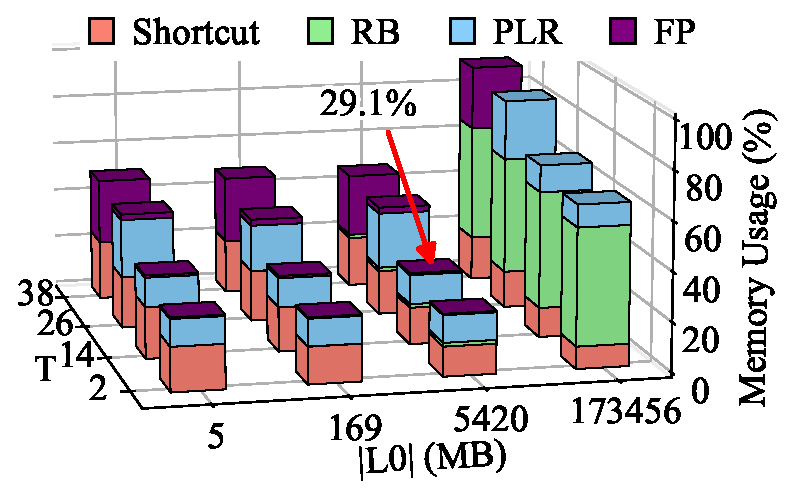
\includegraphics[width=\textwidth]{figs/Figure_lsm_design/lsm_design/3d_memory/3d_memory2.eps}
         \caption{Memory usage depending $T$ and $|L_0|$}
     \end{subfigure}
     \hfill
     \begin{subfigure}[b]{0.28\textwidth}
         \centering
         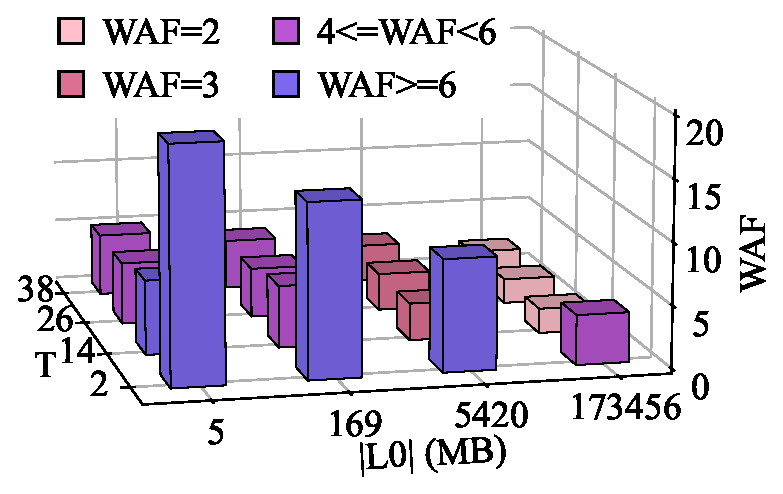
\includegraphics[width=\textwidth]{figs/Figure_lsm_design/lsm_design/3d_waf/3d_waf_2.eps}
         \caption{WAF depending $T$ and $|L_0|$}
     \end{subfigure}

	 \caption{Memory and performance analysis of \ours{} depending on tree organization}
\label{fig:tree-org}
\end{figure*}
\end{comment}

\begin{comment}
\begin{figure*}[t]
     \centering
     \begin{subfigure}[b]{0.175\textwidth}
         \centering
         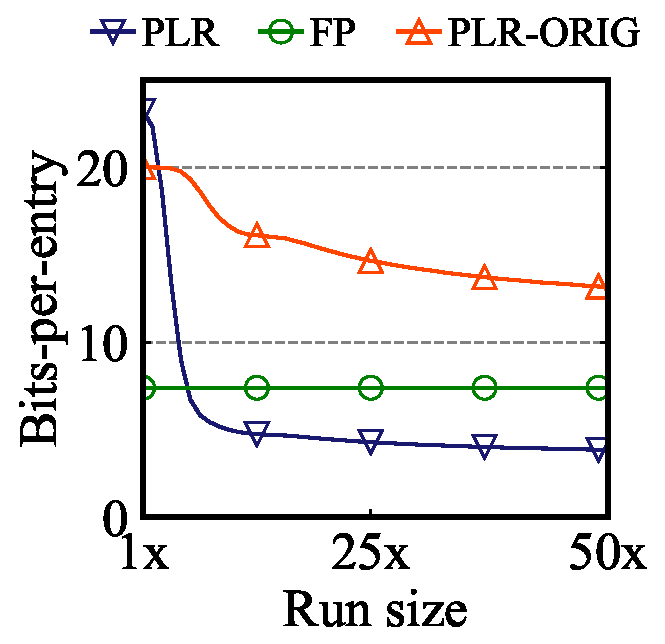
\includegraphics[width=\textwidth]{figs/Figure_lsm_design/lsm_design/BF-PLR/OURS-BF-PLR.eps}
         \caption{\# of bits per entry}
         \label{fig:tree-org}
     \end{subfigure}
     \hfill
     \begin{subfigure}[b]{0.28\textwidth}
         \centering
         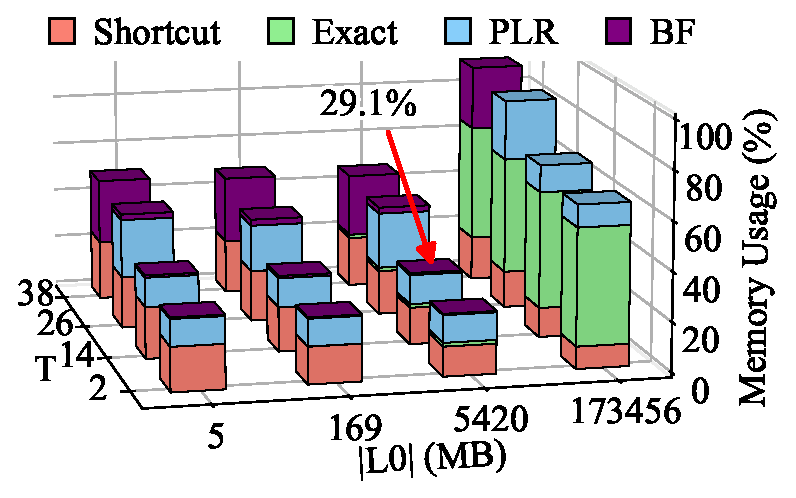
\includegraphics[width=\textwidth]{figs/Figure_lsm_design/lsm_design/3d_memory/3d_memory.eps}
         \caption{Memory usage depending $T$ and $|L_0|$}
         \label{fig:tree-org}
     \end{subfigure}
     \hfill
     \begin{subfigure}[b]{0.28\textwidth}
         \centering
         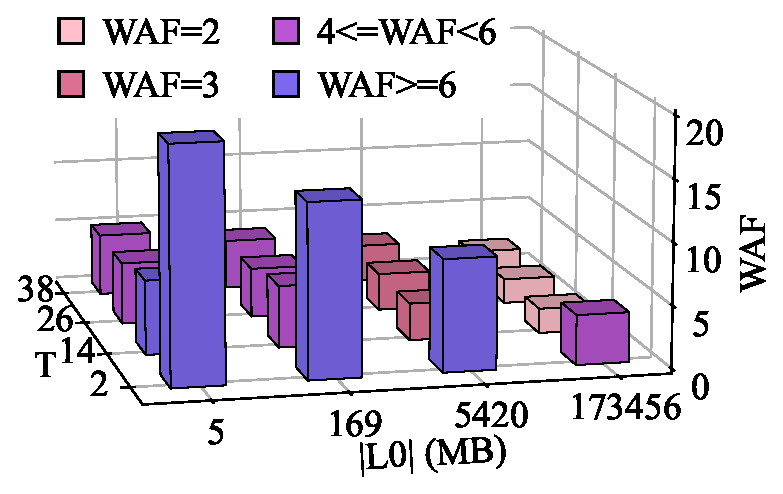
\includegraphics[width=\textwidth]{figs/Figure_lsm_design/lsm_design/3d_waf/3d_waf_2.eps}
         \caption{WAF depending $T$ and $|L_0|$}
         \label{fig:tree-org}
     \end{subfigure}
     \hfill
     \begin{subfigure}[b]{0.202\textwidth}
         \centering
         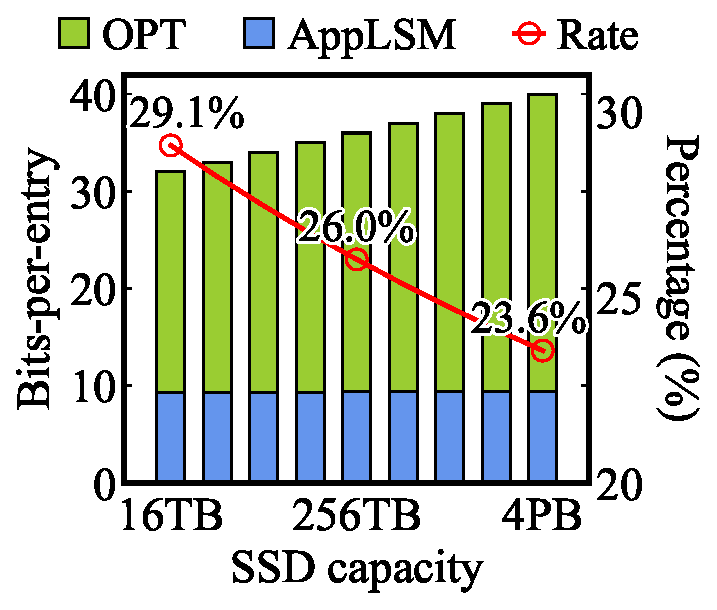
\includegraphics[width=\textwidth]{figs/Figure_lsm_design/lsm_design/scale/twinx-scale.eps}
         \caption{Scalability w/ SSD size}
         \label{fig:tree-org}
     \end{subfigure}
	 \vspace{-10pt}
	 \caption{Memory and performance analysis of \ours{} depending on tree organization, \FIXME{BF-->FP, add PLR original to (a)}}
	 \vspace{-10pt}
\label{fig:tree-org}
\end{figure*}
\end{comment}


%In this section, we explore the optimal organization of the LSM-tree to maximize
%the memory efficiency of both the BF- and PLR-based indexing algorithms when
%they are used together.  
In this section, we explore the organization of an LSM-tree and analyze
its impact on the memory usage when FP and PLR are used together.  
The tree organization also has a high impact on
write performance since WAF varies depending on a tree height $h$
as we mentioned before (see~\SEC{sec:back:lsm-tree}).  
We discuss how to derive a balanced tree hierarchy that
satisfies both memory efficiency and high write throughput.

\begin{comment}
The two approximate algorithms 
show different performance and memory usages depending on which level they are assigned. 
This section
explores how the optimal tree organization can be derived in a manner
that minimizes the memory requirement. We also consider the
impact of the tree organization on the write amplification factor (WAF)
($=\frac{\text{data written to flash}}{\text{data written by host}}$).
\end{comment}


%\st{\textbf{Impact of tree organization on memory.}}
%\JS{\textbf{Impact of run size on approximate indexing techniques.}}
\begin{comment}
As discussed in \SEC{sec:design:bf-plr-basic}, 
the PLR-based indexing provides high memory efficiency when a run size is large.  
%As the run gets larger, mapping pairs are likely to be more densely sorted within the run,
%which enables us to express many entries using fewer equations. 
Conversely, regardless of the run size, the BF-based indexing requires the same number of bits
per entry. This is because a BF entry size is decided by a target
FPR and the number of BFs to be tested (see \EQ{eq:fpr-relax}). Those parameters are decided at the design time
(\eg~$FPR_{T}$=0.1 and $n$=28 in \SEC{sec:opt:memory}) and 
are the same for all the runs. 
We plot the number of bits per mapping entry while varying the run size (the
unit run size is 10GB and the storage capacity is 1TB) in
\FIG{fig:tree-org}(a).  For small runs, the BF-based indexing is better, but as the
run size grows, the PLR achieves better memory
efficiency.  
%\todo{
Given a specific tree, we can achieve the best memory efficiency
by assigning one (either BF- or PLR-based indexing) 
that requires less memory to each level.
%make it decide which
%algorithms should be assigned to which layer; we just need to choose the most memory
%efficient one. (이러한 분위기로...)}
%It also shows how better memory-optimized it is compared to the
%original PLR (denoted as \texttt{PLR(ORIG)}).  
\end{comment}

Our results in \SEC{sec:combine} suggests that
it is desirable to increase the average run size if possible.
It may increase the likelihood that more runs are managed 
by memory-efficient PLR models.
%further reducing the memory usage of the tree.
Let $R_{avg}$ be the average run size in the tree.
$R_{avg}$ is obtained by dividing the storage capacity ($CAP$)
by the total number $r_{tot}$ of runs in the tree. In \ours{}, the
top level $L_0$ has a single run (see~\SEC{design:overall}). From $L_1$ to $L_{h-1}$, the
number $r$ of runs per level is the same. If the tree height is
$h$, $r_{tot}$ is $(h-1) \cdot r + 1$. 
$R_{avg}$ is thus defined as follows:
\begin{equation}
\small
\begin{split}
	R_{avg}=\frac{CAP}{(h-1) \cdot r + 1}.
\end{split}
\label{eq:r_avg_original}
\end{equation}

By reducing $h$ and $r$, we make $R_{avg}$ larger. 
Changing the run size is not easier than it appear to be.
This is because $h$ and $r$ are also decided by two tree parameters,
(\textit{i}) the size factor $T$ and (\textit{ii}) the size of $L_{0}$, 
which affect the memory usages of other components, 
the RB-tree for $L_0$ and the shortcut table.
%Thus, we should choose the proper $T$ and size of $L_0$ considering their impacts.
%on performance and memory.

%I/O performance and 
%total memory usage of \ours{}.
%To figure out the relationship among $R_{avg}$, I/O performance and the total memory requirement, 
%we reorganize \EQ{eq:r_avg_original} by using $T$ and size of $L_0$.


Let us express $h$ using the size factor $T$ and the size of $L_0$.
%\st{To obtain $h$, let}\JS{First, we define $h$ by the two variables. Let} 
Let $|L_i|$ be the size of $L_i$ in the tree.
$|L_i|$ increases by a factor of $T$ from the
top-level $L_0$, that is, $|L_{i}| = |L_0| \cdot T^{i}$ ($0<i<h$), where $i$ is
the level number.  $h$ 
%the level number and $h$ is the tree height.  $h$ 
is thus defined as follows (detailed derivation steps are given in~\cite{monkey}):
\begin{equation}
\small
\begin{split}
	h &= \ceil*{log_{T}\left(\frac{CAP}{|L_0|} \right)}.
\end{split}
\label{eq:n_level}
\end{equation}
\begin{comment}
\st{where $C$ is the SSD capacity.}
%If $C$ = 1 TB, $|L_0|$ = 256 MB, and
%$T$ = 4, $h = 6$. 
\st{Since $C$ is fixed in our setup, $|L_0|$ and $T$ decide
the tree height $h$. 
As $L_0$ and $T$ get larger, the tree becomes fatter and $h$ becomes smaller, 
and vice versa.}
%As will be discussed later, the tree height has a high impact on WAF.
\end{comment}

%$T$ also represents the number $N_{run}$ of runs per level in \ours{}.
%\st{$T$ decides the number $N_{run}$ of runs per level.}
In LSM-trees, $r = T$.  The proof is straightforward.  For compaction
of $L_i$ and $L_{i+1}$, \ours{} reads all the runs $R_i$ at $L_i$, merges and
sorts data, and write them to $L_{i+1}$, creating a new run $R_{i+1}$.
The size $|R_{i+1}|$ of $R_{i+1}$ is thus equal to $|L_i|$.  For $|L_{i+1}|$ to
be $T$ times larger than $|L_{i}|$, $L_{i+1}$ should have $T$ runs.  
\begin{comment}
\begin{equation}
\small
\begin{split}
	r &= T.
\end{split}
\label{eq:n_run}
\end{equation}
\end{comment}

\begin{figure}[t]
     \centering
     \begin{subfigure}[b]{0.23\textwidth}
         \centering
         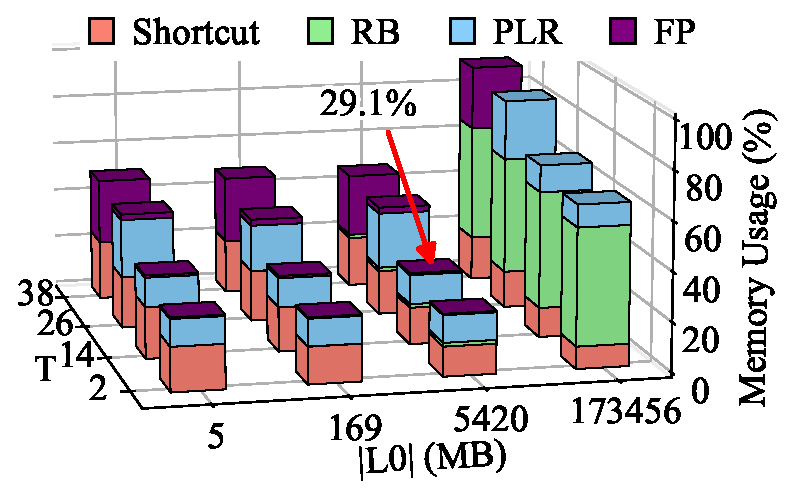
\includegraphics[width=\textwidth]{figs/Figure_lsm_design/lsm_design/3d_memory/3d_memory2.eps}
         \caption{Memory usage}
     \end{subfigure}
     \hfill
     \begin{subfigure}[b]{0.23\textwidth}
         \centering
         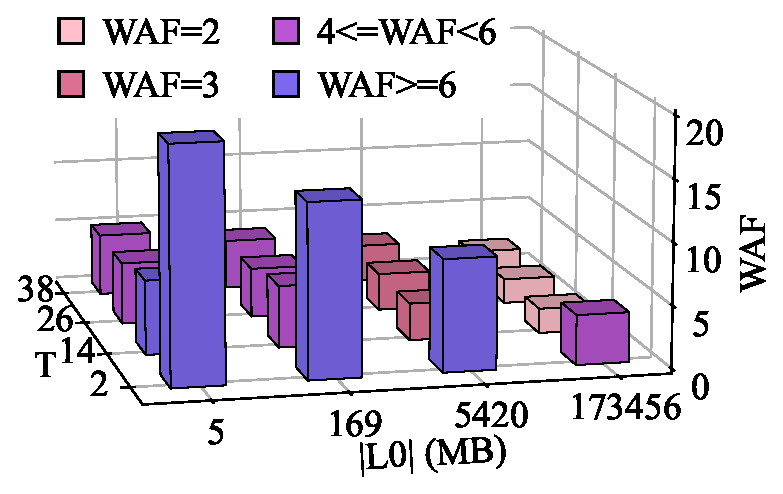
\includegraphics[width=\textwidth]{figs/Figure_lsm_design/lsm_design/3d_waf/3d_waf_2.eps}
         \caption{WAF}
     \end{subfigure}  
     \vspace{-5pt}

	 \caption{Memory usage and WAF depending $T$ and $|L_0|$}
  \vspace{-5pt}
\label{fig:tree-org}
\end{figure}

%Using Eqs.~(\ref{eq:n_level}) and~(\ref{eq:n_run}), 
Using Eq.~(\ref{eq:n_level}), \EQ{eq:r_avg_original} can be 
rewritten as follows:
\begin{equation}
\small
\begin{split}
	R_{avg} &= \frac{CAP}{(h-1) \cdot r + 1} = \frac{CAP}{(\ceil*{log_{T}\left(\frac{CAP}{|L_0|} \right)}-1)\cdot T+1}.
\end{split}
\label{eq:r_avg}
\end{equation}

\EQ{eq:r_avg} tells us that $R_{avg}$ can be increased 
by reducing $T$ and increasing $|L_0|$, and vice versa.

We measure the memory usage
and WAF of \ours{} while varying $T$ and $|L_0|$,
\FIG{fig:tree-org}(a) illustrates the memory usage (\%) of
\ourtree{}, relative to the optimal FTL.
We break down the graph to highlight
the memory usage of four key components:
FPs, PLR models, the RB-tree for $L_0$, 
and the shortcut table.  
For each level, either the FP- or
PLR-based indexing can be used.  We choose one that requires less memory.  

We
make two key observations.  First, the memory requirement 
is mainly decided by $T$.  The smaller $T$, the larger the memory
savings as a run gets larger in size.
As $T$ increases, the memory efficiency of PLR rapidly drops, and
at $T=38$, PLR is no longer useful. % owing to the small run size.
Instead, using FP is more beneficial.  Additionally, 
the shortcut table size is proportional to $r$, 
it gets smaller as $T$ reduces.
Second, the size of $L_0$ has a negligible impact on memory
usage. By increasing $|L_0|$, we can make 
$R_{avg}$ larger.
However, since $R_{avg}$ increases logarithmically as $|L_0|$,
its impact is not huge.
However, when $L_0$ increases too large, 
the RB-tree consumes lots of DRAM.

\FIG{fig:tree-org}(a) displays the WAFs of the trees for the same combinations
of $T$ and $L_0$ in \FIG{fig:tree-org}(b).  
%In LSM-trees, whenever compaction is triggered, valid data stored
%in $L_i$ are copied to a new run in the
%next level, $L_{i+1}$. 
%As the tree becomes taller, the compaction cost gets higher
%because compaction is more frequently invoked~\cite{monkey}.
%As a result, the WAF of \ourtree{} is directly proportional
%to $h$ in \EQ{eq:n_level}. \FIG{fig:tree-org}(d)  supports this fact well;
According to \EQ{eq:n_level},
as $T$ and/or $L_0$ get smaller, the tree becomes taller,
which results in an increase of $h$.
As mentioned in \SEC{sec:back:lsm-tree}, with higher $h$, 
the overall WAF of the tree increases.

From Figs.~\ref{fig:tree-org}(a) and (b), we notice that there exists a
trade-off between the memory and WAFs.  To minimize the memory requirement, it
is preferred to set $T$ very small with a balanced $|L_0|$.  
But, for write throughput, 
setting $T$ and $|L_0|$ very large is a good choice.
However, in most cases, a balanced tree would be preferred.  
When $T=14$ and $|L_0|$ = 5.4GB, \ourtree{} reduces the memory
space to 29.1\% compared to the optimal FTL 
with the reasonable WAF of 3.  With the balanced option,
\ours{} is organized with three levels: 
$L_0$ with RB-tree, $L_1$ with FP indices, and $L_2$ with PLR models.

\begin{comment}
\todo{(실험 결과에 넣는것이 좋을 듯)}

\textbf{Scalability issue:}
As SSD capacity increases, each entry of the typical index table requires more
bits because it has to cover larger physical space.  For a 16TB SSD, a 32-bit
table entry is enough, but it increases to 35-bit when an SSD size
increases to 128TB.  The number of entries per table increases as well.
Compared to typical FTLs, \ours{} provides better scalable in terms of memory.
By increasing a run size, we can keep using the balanced setup,
regardless of SSD capacity.  The tree parameters, $T$, $h$, and $r$, remain the
same.  To cover larger physical space, the number of FP indices and PLR
equations in the tree increases, but the number of bits per FP-entry and
PLR-equation does not.  As pointed out before, the FP size is decided by
\JS{$\mathcal{E}_{FP}$ and $k$}.  \fixme{$x_0^i$ and $y_0^i$ of $S_i$} increase, but since they are
delta-encoded over sorted fragments, we can express them using the same
number of bits (\ie~11-bit and 9-bit).  
%\sout{Only the
%exceptions are the exact indices for $L_0$, guards of BF-indexing that point
%to exact locations $y_i$ of physical sectors.}
Only the exceptions are the \JS{RB-tree} for $L_0$, \JS{the first entries of FP groups 
and delta-encoded PLR groups}.
However, since the \JS{RB-tree} and the FP-based indexing occupy
only about 5\% of the total memory usage (see \FIG{fig:tree-org}(c)) and
the pivots occupy 0.06\%, their
impacts on the total memory are negligible.  \FIG{fig:scalability} compares the
number of bit per entry of the optimal FTL and \ours{}.  The optimal FTL needs
more bits per entry as the SSD capacity gets larger, but \ours{} has almost the
same bits per entry, exhibiting better scalability.
\end{comment}

\subsection{Crash Consistency}
Approximate indices that reside in
DRAM are immutable and thus all clean. The loss of them
on a crash does not make the system inconsistent. The
memtable, the shortcut table, and the RB-tree, however,
keep dirty indices and data in memory, 
so their loss may lead to the inconsistent system.
The loss of buffered data in the memtable is inevitable 
(unless it is backed by capacitors), but
it does not hurt consistency like other log-structured systems.  
The RB-tree is rebuilt by scanning small $L_0$ 
as LBAs of data are recorded in OOBs. 
However, the reconstruction of the shortcut table is challenging
as it takes so long to scan the entire tree.  
To address this, when the memtable is flushed out to $L_0$ 
or runs are compacted with the next level,
\ours{} writes associated shortcut-table entries to run's metadata.
During recovery, 
we can quickly rebuild the shortcut table 
by reading run's metadata.



\begin{comment}
\JS{
This balanced tree setup can be adopted to any storage capacities by scaling $|L_{0}|$.
If \ours{} has the same values of $\frac{C}{|L_0|}$ and $T$ in different storage capacities, 
it has the similar I/O performance and memory requirement (see Eq.~(\ref{eq:n_level}) and (\ref{eq:r_avg})).
Some data structures (\ie~guard of BF-indexing and exact indexing for $L_0$) 
may need more bits than 32-bit as the physical storage gets larger.
However, they occupies only about 5\% of the total memory usage in balanced tree setup as shown in \FIG{fig:tree-org}(b).
Thus, the effects of these data structures on the total memory are negligible.
\FIG{fig:tree-org}(d) shows the impact of storage capacities on the \ours{}
memory usage with balanced tree parameters and 0.1 FPR.
The optimal FTL needs more bits per entry as the storage capacity gets larger, but 
\ours{} has almost the same bit per entry. 
As a result, the memory usage ratio between \ours{} and the optimal FTL goes down.
}
%For read-only applications where write
%throughput is not as important, 
%the tree with smaller $T$ and $L_0$ might be better.  Conversely, for write-heavy applications, we have to trade memory for
%lower WAF. 
\end{comment}

\begin{comment}
Once tree organization is decided, we can fine-tune RAF
and memory by changing FPR. By increasing FPR, we further reduce the memory
requirement, sacrificing read latency, and vice versa.  \FIG{fig:tree-org}(d)
is the memory usage by FPR. 
\end{comment}
